\chapter{Other One- and Three-Dimensional Waves}

Having developed the machinery of normal modes, travelling solutions, and Fourier decomposition on the string, we can now let the same wave equation loose on the rest of physics. The remarkable fact is that it reappears almost unchanged in system after system, asking only that we reinterpret its symbols: the transverse displacement of a string becomes the longitudinal displacement of a gas parcel, or a component of the electric field, or the charge density of a plasma. In this chapter we follow that thread through longitudinal sound waves in a gas and electromagnetic waves in vacuum and in matter, and we use them to understand dispersion, polarization, reflection, refraction, and radiation. Along the way the one-dimensional string is generalized to two and three spatial dimensions, and the Fourier series is sharpened into the continuous Fourier transform.

% ============================================================
\section{Sound Waves}
% ============================================================

Recall that a transverse wave $y(x,t)$ on a string of linear density $\rho_L$ and tension $T$ carries kinetic and potential energies
\begin{equation}
    \mathrm{KE} = \int_0^L \tfrac{1}{2}\rho_L\left(\pdv{y}{t}\right)^2 dx, \qquad
    \mathrm{PE} = \int_0^L \tfrac{1}{2} T\left(\pdv{y}{x}\right)^2 dx.
\end{equation}
Sound is the natural longitudinal analogue. Instead of a transverse displacement $y$ perpendicular to the direction of travel, we track the \emph{longitudinal} displacement $\psi(x,t)$ of the fluid parcel whose equilibrium position is $x$: the parcel is nudged back and forth along the very direction the wave propagates. The restoring ``tension'' will turn out to be the gas's own resistance to being compressed.

\subsection{Setup}

Consider a long tube of cross-sectional area $A$ filled with a gas of equilibrium pressure $p_0$ and density $\rho$. Focus on a thin slab of gas lying between $x$ and $x + \ell$, with equilibrium volume $V = A\ell$. When the wave passes, the left face is displaced to $x + \psi(x,t)$ and the right face to $x + \ell + \psi(x + \ell, t)$, as sketched in Figure~\ref{fig:sound-slab}. The slab's new volume is
\begin{equation}
    V + \Delta V = A\bigl(\ell + \psi(x+\ell, t) - \psi(x,t)\bigr),
\end{equation}
so, in the limit $\ell \to 0$,
\begin{equation}
    \Delta V \;\approx\; A\,\pdv{\psi}{x}\,\ell.
\end{equation}

\begin{figure}[H]
\centering
\begin{tikzpicture}[>=Stealth,scale=1]
  \fill[LightGreen] (3,0) rectangle (5,1.8);
  \fill[LightOrange,opacity=0.7] (3.7,0) rectangle (6.1,1.8);
  \draw[thick] (0,0)--(9.2,0);
  \draw[thick] (0,1.8)--(9.2,1.8);
  \draw[dashed] (3,-0.15)--(3,1.95);
  \draw[dashed] (5,-0.15)--(5,1.95);
  \draw[thick] (3.7,0)--(3.7,1.8);
  \draw[thick] (6.1,0)--(6.1,1.8);
  \draw[->] (3,-0.4)--(3.7,-0.4) node[midway,below]{\small$\psi(x)$};
  \draw[->] (5,2.15)--(6.1,2.15) node[midway,above]{\small$\psi(x+\ell)$};
  \node at (2.75,0.9){\small$x$};
  \node at (5.0,0.9){\small$x{+}\ell$};
  \node at (8.7,1.3){\small propagation};
  \draw[->,thick] (8.3,0.9)--(9.1,0.9);
\end{tikzpicture}
\caption{A slab of gas (green, equilibrium) between $x$ and $x+\ell$ is displaced and stretched by a passing sound wave (orange). Because the right face moves farther than the left, the slab's volume changes by $\Delta V \approx A\,(\partial_x\psi)\,\ell$; this compression or rarefaction is what changes the local pressure.}
\label{fig:sound-slab}
\end{figure}

The displacement can do two quite different things. A \emph{uniform} translation ($\partial_x\psi = 0$) merely slides the slab bodily and is dynamically harmless. Only a nonzero $\partial_x\psi$ stretches or squeezes it, and it is this compression or rarefaction that changes the local pressure through the equation of state.

\subsection{Adiabatic Equation of State}

Sound waves compress and rarefy the gas so rapidly that heat has no time to flow between neighbouring parcels. The process is therefore \emph{adiabatic}, obeying
\begin{equation}
    p V^\gamma = \text{const}, \qquad \gamma = \frac{c_p}{c_v}.
\end{equation}
For diatomic gases in air, $\gamma = 7/5$. If the equilibrium state satisfies $p_0 V_0^\gamma = \text{const}$, then a perturbed state obeys $(p_0 + \Delta p)(V_0 + \Delta V)^\gamma = p_0 V_0^\gamma$. Taylor-expanding $(1 + \Delta V/V_0)^\gamma \approx 1 + \gamma\,\Delta V/V_0$ and dropping the second-order product $\Delta p\,\Delta V$,
\begin{equation}
    0 = \Delta p\, V_0^\gamma + p_0\gamma\, V_0^{\gamma-1}\Delta V
    \quad\Longrightarrow\quad
    \Delta p = -\frac{p_0\gamma\,\Delta V}{V_0} = -\gamma p_0\,\pdv{\psi}{x}.
\end{equation}
The pressure field is therefore
\begin{formula}
\begin{equation}
    p(x,t) = p_0 - \gamma p_0\,\pdv{\psi}{x}.
\end{equation}
\end{formula}
Compressions ($\partial_x\psi < 0$) raise the pressure; rarefactions ($\partial_x\psi > 0$) lower it, exactly as intuition demands.

\subsection{Newton's Second Law for the Slab}

The slab is pushed on its left face and its right face by the surrounding gas; the net force is $A[\Delta p(x,t) - \Delta p(x+\ell,t)]$, and its mass is $m = \rho\, A\,\ell$. In the limit $\ell \to 0$,
\begin{equation}
    F_{\text{net}} = -A\,\pdv{\Delta p}{x}\,\ell = m\,\ddot\psi
    \quad\Longrightarrow\quad
    \rho\,\ell A\,\ddot\psi = A\,\ell\, \gamma p_0\,\pdv[2]{\psi}{x}.
\end{equation}
Cancelling the common factor $A\ell$ leaves the sound-wave equation:
\begin{formula}
\begin{equation}
    \pdv[2]{\psi}{t} = \frac{\gamma p_0}{\rho}\,\pdv[2]{\psi}{x},
    \qquad v_p = \sqrt{\frac{\gamma p_0}{\rho}}.
\end{equation}
\end{formula}
This is precisely the transverse string equation in disguise, with $\gamma p_0$ playing the role of tension and $\rho$ the role of mass density. Every technique we developed for the string --- normal modes, travelling solutions, superposition --- carries over verbatim.

\subsection{Normal Modes in a Tube}

As a first application, consider a tube closed at $x=0$ and open at $x=L$. Every normal-mode solution has the standing-wave form
\begin{equation}
    \psi = \sum_{m=1}^\infty A_m \sin(k_m x + \alpha_m)\sin(\omega_m t + \beta_m),
\end{equation}
and the two ends impose the boundary conditions. At the closed end the gas cannot move, so $\psi(0,t) = 0$, forcing $\alpha_m = 0$. At the open end the pressure must match the atmosphere, $\Delta p(L,t) = 0$, which by the pressure formula means $\partial_x\psi(L,t) = 0$. Hence
\begin{equation}
    \cos(k_m L) = 0 \quad\Longrightarrow\quad k_m = \frac{(m - 1/2)\pi}{L}.
\end{equation}
Only odd harmonics survive --- the characteristic timbre of a stopped organ pipe, which sounds an octave lower than an open pipe of the same length.

\subsection{Degrees of Freedom and \texorpdfstring{$\gamma$}{gamma}}

The one microscopic input to the sound speed is $\gamma$, and it is fixed by counting the ways a molecule can store energy: $\gamma = (f+2)/f$, where $f$ is the number of accessible degrees of freedom per molecule.

\begin{fact}[Equipartition]
Each quadratic degree of freedom contributes $\tfrac{1}{2}k_B T$ to the internal energy. A molecule has $f = 3$ translational degrees (always), $f = 2$ additional rotational degrees at moderate temperatures (for non-monatomic molecules), and $2(3N-5)$ vibrational degrees (each vibration counts twice, kinetic and potential) at high temperatures for an $N$-atom molecule.
\end{fact}
For diatomic air near room temperature the rotational modes are active but the vibrational ones are frozen out, giving $f = 5$ and $\gamma = 7/5$, in agreement with measured sound speeds.

% ============================================================
\section{Electromagnetic Waves in Vacuum}
% ============================================================

We now make the boldest of these reinterpretations: the wave medium disappears entirely, and the oscillating quantity becomes the electromagnetic field itself. Maxwell's equations, in SI units and in free space, are
\begin{equation}
    \div \vect{E} = \frac{\rho}{\varepsilon_0}, \qquad
    \div \vect{B} = 0, \qquad
    \curl \vect{E} = -\pdv{\vect{B}}{t}, \qquad
    \curl \vect{B} = \mu_0\!\left(\vect{J} + \varepsilon_0\,\pdv{\vect{E}}{t}\right).
\end{equation}
Here $\mu_0$ is the permeability of free space and $\varepsilon_0$ the permittivity. In vacuum there are no sources, so $\rho = 0$ and $\vect{J} = 0$.

\subsection{Deriving the Wave Equation}

The trick is to decouple $\vect{E}$ and $\vect{B}$ by taking a second curl. Applying $\curl$ to Faraday's law and using the identity $\curl(\curl\vect{A}) = \grad(\div\vect{A}) - \laplacian \vect{A}$,
\begin{equation}
    \curl\curl\vect{E} = \grad(\div\vect{E}) - \laplacian\vect{E} = -\laplacian\vect{E},
\end{equation}
since $\div\vect{E} = 0$ in vacuum. On the other hand, substituting the Ampère--Maxwell law for $\curl\vect{B}$,
\begin{equation}
    \curl\curl\vect{E} = -\pdv{}{t}(\curl\vect{B}) = -\mu_0\varepsilon_0\,\pdv[2]{\vect{E}}{t}.
\end{equation}
Equating the two expressions,
\begin{formula}
\begin{equation}
    \pdv[2]{\vect{E}}{t} = \frac{1}{\mu_0\varepsilon_0}\,\laplacian\vect{E}.
\end{equation}
\end{formula}
An identical argument gives $\partial_t^2\vect{B} = (\mu_0\varepsilon_0)^{-1}\laplacian\vect{B}$. Each Cartesian component of $\vect{E}$ and $\vect{B}$ thus satisfies the three-dimensional wave equation, with phase speed
\begin{equation}
    c = \frac{1}{\sqrt{\mu_0\varepsilon_0}} \approx 3\times 10^8\ \mathrm{m/s}.
\end{equation}
That the speed of light emerges from two constants measured in the laboratory with capacitors and coils --- with no reference to light at all --- was Maxwell's decisive discovery, and the first hint that optics is a branch of electromagnetism.

\subsection{Plane-Wave Solutions}

Consider the simplest solution: a wave polarized along $\hat{x}$ and travelling along $\hat{z}$,
\begin{equation}
    \vect{E} = \operatorname{Re}\bigl(E_0 e^{i(kz - \omega t)}\hat{x}\bigr) = E_0 \cos(kz - \omega t)\,\hat{x}.
\end{equation}
Substituting into the wave equation gives $-E_0 k^2 \cos(kz-\omega t)\,\hat{x} = -\mu_0\varepsilon_0 E_0 \omega^2 \cos(kz-\omega t)\,\hat{x}$, so
\begin{formula}
\begin{equation}
    \omega = \frac{k}{\sqrt{\mu_0\varepsilon_0}} = c k.
\end{equation}
\end{formula}
This is the vacuum dispersion relation: linear, and hence non-dispersive --- every frequency travels at the same speed $c$. The magnetic partner is fixed by Faraday's law $\curl\vect{E} = -\partial_t\vect{B}$, which yields
\begin{equation}
    \vect{B}(\vect{r},t) = \frac{1}{c}\,\hat{k}\times \vect{E},
\end{equation}
valid \emph{only} for travelling waves. The field structure is shown in Figure~\ref{fig:em-planewave}: $\vect{E}$ and $\vect{B}$ are mutually perpendicular, both perpendicular to the direction of travel, and oscillate exactly in phase.

\begin{figure}[H]
\centering
\begin{tikzpicture}[>=Stealth,scale=1]
  \draw[->,thick] (0,0,0) -- (11,0,0) node[right]{$z$};
  \draw[->] (0,-2.3,0) -- (0,2.7,0) node[above]{$x,\ \vect{E}$};
  \draw[->] (0,0,-2.3) -- (0,0,2.6) node[below left]{$y,\ \vect{B}$};
  \draw[red,thick,domain=0:10.8,samples=90,variable=\t] plot ({\t},{1.8*sin(\t r)},{0});
  \draw[blue,thick,domain=0:10.8,samples=90,variable=\t] plot ({\t},{0},{1.8*sin(\t r)});
  \foreach \t in {0.6,1.4,...,10.6} {
    \draw[red,->] (\t,0,0) -- (\t,{1.8*sin(\t r)},0);
    \draw[blue,->] (\t,0,0) -- (\t,0,{1.8*sin(\t r)});
  }
\end{tikzpicture}
\caption{A snapshot of a linearly polarized plane wave travelling along $\hat{z}$. The electric field $\vect{E}$ (red) oscillates along $\hat{x}$ and the magnetic field $\vect{B}$ (blue) along $\hat{y}$; the two are perpendicular, in phase, and related by $\vect{B} = \hat{k}\times\vect{E}/c$.}
\label{fig:em-planewave}
\end{figure}

\subsection{General Plane Wave}

More generally, a plane wave travelling in an arbitrary direction is
\begin{equation}
    \vect{E}(\vect{r},t) = \operatorname{Re}\bigl[\vect{E}_0\, e^{i(\vect{k}\cdot\vect{r} - \omega t + \phi)}\bigr],
\end{equation}
where $\vect{E}_0 = \langle E_{0x}, E_{0y}, E_{0z}\rangle$ specifies the polarization, $\vect{k} = \langle k_x, k_y, k_z\rangle$ the direction of propagation, and $|\vect{k}| = 2\pi/\lambda$. The magnetic field is again
\begin{equation}
    \vect{B}(\vect{r},t) = \frac{1}{c}\hat{k}\times \vect{E}(\vect{r},t).
\end{equation}

\begin{example}[Wave at $45^\circ$ in the $xy$-plane]
Suppose $|\vect{k}| = 2\pi/\lambda$ points at $45^\circ$ in the $xy$-plane, so
\begin{equation}
    \vect{k} = \frac{\sqrt{2}\pi}{\lambda}\begin{pmatrix}1\\1\\0\end{pmatrix}.
\end{equation}
Since $\vect{E}\perp\hat{k}$ and lies in the $xy$-plane, one valid choice is $\vect{E} = E_0\langle -\tfrac{1}{\sqrt 2}, \tfrac{1}{\sqrt 2}, 0\rangle\cos\!\left(\tfrac{\pi\sqrt 2}{\lambda}(x+y) - \omega t + \phi\right)$, and the magnetic field is $\vect{B} = (E_0/c)\,\hat{z}\cos(\cdots)$, perpendicular to both.
\end{example}

\subsection{Transverseness of EM Waves}

The perpendicularity we drew in Figure~\ref{fig:em-planewave} is not an accident of the special case but a theorem forced by Maxwell's equations.

\begin{theorem}[Transverseness]
For a plane wave $\vect{E} = \vect{E}_0 e^{i(\vect{k}\cdot\vect{r} - \omega t)}$ in vacuum,
\begin{equation}
    \vect{E}_0\cdot\vect{k} = 0, \qquad \vect{B}_0\cdot\vect{k} = 0.
\end{equation}
Furthermore $\vect{E}\perp\vect{B}$ and $|\vect{E}| = c|\vect{B}|$.
\end{theorem}

\emph{Proof.} From $\div\vect{E} = 0$,
\begin{equation}
    \div \vect{E} = i(\vect{E}_0\cdot\vect{k})e^{i(\vect{k}\cdot\vect{r} - \omega t)} = 0
    \;\Longrightarrow\; \vect{E}_0\cdot\vect{k} = 0,
\end{equation}
and the proof for $\vect{B}_0$ from $\div\vect{B} = 0$ is identical. From Faraday's law $\vect{k}\times\vect{E}_0 = \omega\vect{B}_0$: since $\vect{k}\perp\vect{E}_0$, one has $\vect{B}_0\perp\vect{E}_0$, and taking magnitudes, $|\vect{k}||\vect{E}_0| = \omega|\vect{B}_0|$ gives $|\vect{E}_0| = c|\vect{B}_0|$. \qed

% ============================================================
\section{Energy and Momentum of EM Waves}
% ============================================================

If light is a wave, it should carry energy and momentum, and we can compute both directly from the fields.

\subsection{Energy Density}

The energy stored per unit volume in the electric and magnetic fields is
\begin{equation}
    u_E = \tfrac{1}{2}\varepsilon_0|\vect{E}|^2, \qquad
    u_B = \frac{1}{2\mu_0}|\vect{B}|^2.
\end{equation}
For a plane wave $|\vect{B}| = |\vect{E}|/c$ and $\mu_0 = 1/(\varepsilon_0 c^2)$, so
\begin{equation}
    u_B = \frac{\varepsilon_0 c^2}{2}|\vect{B}|^2 = \tfrac{1}{2}\varepsilon_0|\vect{E}|^2 = u_E.
\end{equation}
The electric and magnetic contributions are exactly equal --- the energy is shared evenly between them --- and the total is
\begin{formula}
\begin{equation}
    u = u_E + u_B = \varepsilon_0|\vect{E}|^2.
\end{equation}
\end{formula}

\subsection{Poynting Vector and Intensity}

To find how fast this energy flows, note that in a time $\Delta t$ the wave advances a distance $c\,\Delta t$, so the energy crossing an area $A$ is $u \cdot A c\,\Delta t$. The flux (energy per unit area per unit time) is $S = c\,\varepsilon_0|\vect{E}|^2 = c^2\varepsilon_0|\vect{E}||\vect{B}|$. Since the flow points along $\vect{E}\times\vect{B}$, we package magnitude and direction into the \emph{Poynting vector}
\begin{formula}
\begin{equation}
    \vect{S} = \frac{\vect{E}\times\vect{B}}{\mu_0}, \qquad |\vect{S}| = c\,\varepsilon_0|\vect{E}|^2,
\end{equation}
\end{formula}
with units of power per unit area ($\mathrm{W/m^2}$).

\begin{definition}[Intensity]
The intensity is the time-averaged magnitude of the Poynting vector. For a plane wave the field oscillates as a cosine, so we average $\langle\cos^2\rangle = \tfrac12$:
\begin{equation}
    I = \langle |\vect{S}|\rangle = \frac{c\varepsilon_0}{2}E_0^2.
\end{equation}
\end{definition}

\subsection{Radiation Pressure}

Light also carries momentum, so it presses on whatever absorbs or reflects it. A photon of energy $u$ carries momentum $p = u/c$; when a beam of intensity $I$ is absorbed by a surface, the momentum delivered per unit area per unit time is
\begin{equation}
    P = \frac{F}{A} = \frac{1}{A}\frac{dp}{dt} = \frac{1}{cA}\frac{du}{dt} = \frac{I}{c}.
\end{equation}
A perfect reflector reverses the photon momentum instead of merely absorbing it, doubling the impulse:
\begin{formula}
\begin{equation}
    \langle P\rangle = \frac{I}{c} \quad\text{(absorption)}, \qquad \langle P\rangle = \frac{2I}{c} \quad\text{(reflection)}.
\end{equation}
\end{formula}

% ============================================================
\section{Reflection off a Perfect Conductor}
% ============================================================

The simplest boundary a wave can meet is a perfect conductor, which rearranges its free charges instantly to cancel any interior electric field. This imposes the boundary condition $\vect{E} = 0$ at the surface. Suppose the conductor fills $z > 0$, and an incident wave
\begin{equation}
    \vect{E}_i = \tfrac{E_0}{2}\cos(kz - \omega t)\hat{x}, \qquad
    \vect{B}_i = \tfrac{E_0}{2c}\cos(kz - \omega t)\hat{y}
\end{equation}
approaches from the left. To enforce $\vect{E}(z=0,t) = 0$ for all $t$, we superpose a reflected wave travelling in $-\hat{z}$ with just the right amplitude:
\begin{equation}
    \vect{E}_r = -\tfrac{E_0}{2}\cos(-kz - \omega t)\hat{x}, \qquad
    \vect{B}_r = \tfrac{E_0}{2c}\cos(-kz - \omega t)\hat{y}.
\end{equation}
Adding incident and reflected waves and applying the sum-to-product identities,
\begin{equation}
    \vect{E} = \vect{E}_i + \vect{E}_r = E_0\sin(\omega t)\sin(kz)\,\hat{x},
    \qquad
    \vect{B} = \vect{B}_i + \vect{B}_r = \frac{E_0}{c}\cos(\omega t)\cos(kz)\,\hat{y}.
\end{equation}
The total field is a standing wave. Notice that $\vect{E}$ and $\vect{B}$ are now $90^\circ$ out of phase in both space and time --- when one is maximal the other vanishes --- which is exactly the opposite of a travelling wave, where the two fields march in lockstep.

% ============================================================
\section{Waves in Two and Three Dimensions}
% ============================================================

So far our waves have lived on a line. The wave equation is happy in any number of dimensions, and generalizing it recovers both the standing modes of a cavity and the plane waves of free space.

\subsection{Standing Modes in a Box}

Consider a rectangular box of dimensions $a\times b\times c$ whose walls force the wave to vanish. Any component of a normal-mode standing wave has the separable form
\begin{equation}
    \psi_i = A_i\sin(k_x x + \delta_x)\sin(k_y y + \delta_y)\sin(k_z z + \delta_z)\sin(\omega t + \beta).
\end{equation}
Substituting into the wave equation $\mu_0\varepsilon_0\,\partial_t^2\psi = \laplacian\psi$ ties the frequency to the wavevector,
\begin{formula}
\begin{equation}
    \omega = c\sqrt{k_x^2 + k_y^2 + k_z^2}.
\end{equation}
\end{formula}
The walls at $x=0,a$ require $\sin(k_x\cdot 0) = 0$, so $\delta_x = 0$, and $\sin(k_x a) = 0$, so $k_x = \ell\pi/a$ for integer $\ell$. Identical conditions in $y$ and $z$ quantize the wavevector into discrete triples $(\ell, m, n)$, giving the mode spectrum
\begin{equation}
    \omega_{\ell m n} = v_p\sqrt{\left(\frac{\ell\pi}{a}\right)^2 + \left(\frac{m\pi}{b}\right)^2 + \left(\frac{n\pi}{c}\right)^2}.
\end{equation}

\subsection{Travelling Waves in 3D}

Removing the walls, a generalized travelling wave has the form
\begin{equation}
    \vect{E}(\vect{r},t) = \vect{E}_0\, f(k_x x + k_y y + k_z z - \omega t) = \vect{E}_0\, f(\vect{k}\cdot\vect{r} - \omega t),
\end{equation}
with dispersion relation $\omega = v_p |\vect{k}|$. Surfaces of constant phase $\vect{k}\cdot\vect{r} - \omega t$ are planes perpendicular to $\vect{k}$, which is exactly why such a solution is called a \emph{plane wave}.

% ============================================================
\section{Dispersion Relations, Group and Phase Velocity}
% ============================================================

The vacuum dispersion relation $\omega = ck$ was as simple as could be. In a general medium the relation between frequency and wavenumber is richer, and that richness has a striking consequence: a wave packet can travel at a speed different from its own ripples.

\begin{definition}[Dispersion relation]
The relation $\omega(k)$ connecting angular frequency and wavenumber. A linear dispersion relation $\omega = v_p k$ is \emph{non-dispersive}: all wavelengths travel at the same speed. Any other form is \emph{dispersive}.
\end{definition}

For a travelling wave the \emph{phase velocity} --- the speed of a single crest --- is
\begin{equation}
    v_p = \frac{\omega(k)}{k}.
\end{equation}
To see this, follow a zero of $\sin(kx - \omega t)$: at $t=0$ it sits at $x=0$; at time $t$ it satisfies $kx - \omega t = 0$, so $x = \omega t/k$ and $\Delta x/\Delta t = \omega/k$.

\subsection{Nonlinear Dispersion}

Keeping higher-order stiffness terms in the underlying equation of motion generates wave equations like
\begin{equation}
    \pdv[2]{\psi}{t} = v_p^2\!\left(\pdv[2]{\psi}{x} - \alpha\,\pdv[4]{\psi}{x}\right).
\end{equation}
Plugging in $\psi = A\cos(kx - \omega t)$ gives the dispersion relation
\begin{equation}
    \omega = v_p k\sqrt{1 + \alpha k^2}.
\end{equation}
Now different wavelengths propagate at different speeds, so a wave packet built from many wavelengths spreads and distorts as it travels.

\subsection{Beats and Group Velocity}

To isolate the speed of a packet in the simplest case, superpose two waves with nearly equal frequencies:
\begin{equation}
    \psi_1 = A\sin(k_1 x - \omega_1 t), \qquad \psi_2 = A\sin(k_2 x - \omega_2 t).
\end{equation}
The sum-to-product identity gives
\begin{equation}
    \psi_1 + \psi_2 = 2A\sin\!\left(\frac{k_1 + k_2}{2}x - \frac{\omega_1 + \omega_2}{2}t\right)\cos\!\left(\frac{k_1 - k_2}{2}x - \frac{\omega_1 - \omega_2}{2}t\right).
\end{equation}
A fast oscillation (the sine, at the average frequency) sits inside a slowly varying modulation envelope (the cosine), as in Figure~\ref{fig:beats}. The envelope travels at
\begin{equation}
    v_{\text{pattern}} = \frac{\omega_1 - \omega_2}{k_1 - k_2},
\end{equation}
and in the limit $k_1 \to k_2$ this difference quotient becomes a derivative:
\begin{formula}
\begin{equation}
    v_g \defeq \dv{\omega}{k}.
\end{equation}
\end{formula}

\begin{figure}[H]
\centering
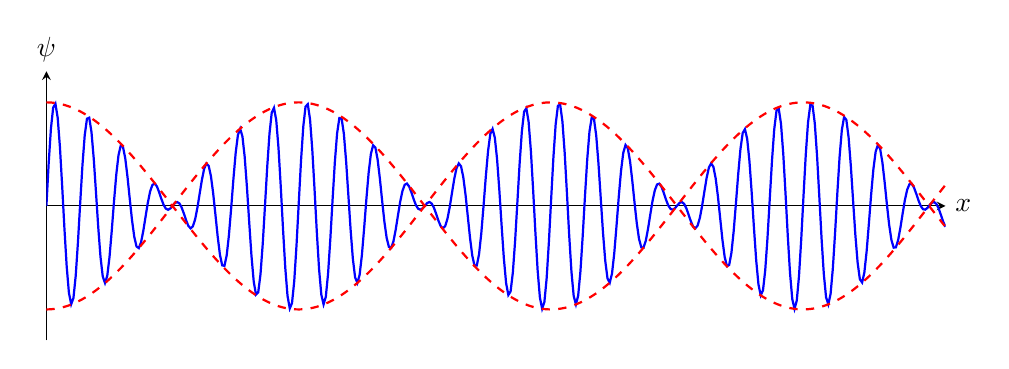
\begin{tikzpicture}
\begin{axis}[width=13cm,height=5cm,axis lines=middle,xtick=\empty,ytick=\empty,
  xlabel={$x$},ylabel={$\psi$},xmin=0,xmax=40,ymin=-2.6,ymax=2.6,samples=400,domain=0:40,
  every axis x label/.style={at={(current axis.right of origin)},anchor=west},
  every axis y label/.style={at={(current axis.above origin)},anchor=south}]
  \addplot[blue,thick]{2*cos(deg(0.28*x))*sin(deg(4.2*x))};
  \addplot[red,dashed,thick]{2*cos(deg(0.28*x))};
  \addplot[red,dashed,thick]{-2*cos(deg(0.28*x))};
\end{axis}
\end{tikzpicture}
\caption{Two waves of nearly equal wavenumber superpose into a fast carrier (blue) modulated by a slow envelope (red dashed). The individual crests move at the phase velocity $v_p = \omega/k$, while the envelope --- and any information it carries --- moves at the group velocity $v_g = \dd\omega/\dd k$.}
\label{fig:beats}
\end{figure}

This is the \emph{group velocity}. Any information encoded in the envelope --- a pulse of light in a fibre, a burst of sound --- travels at $v_g$, not at the phase velocity $v_p$. In a non-dispersive medium the two coincide, $v_g = v_p$; in a dispersive medium they differ, sometimes dramatically.

% ============================================================
\section{Fourier Transform}
% ============================================================

Wave packets like the one above are built by summing many wavelengths, which raises the general question of how to decompose an arbitrary profile into its constituent waves. For an infinite string with no boundary conditions the allowed wavenumbers $k$ are no longer quantized, so the Fourier \emph{series} of the finite string is replaced by a continuous \emph{integral}:
\begin{equation}
    \psi(x, t=0) = \int_{-\infty}^{\infty} c(k)\, e^{ikx}\, dk.
\end{equation}
Given the profile $\psi(x,0)$, how do we extract the amplitude $c(k)$ of each wavenumber?

\subsection{The Dirac Delta and Orthogonality}

The key tool is the Dirac delta, defined by $\delta(x) = 0$ for $x\neq 0$ and $\int_{-\infty}^{\infty}\delta(x)\,dx = 1$, with the sifting property $\int f(x)\delta(x - x_0)\,dx = f(x_0)$. It expresses the orthogonality of the complex exponentials in exactly the form we need:
\begin{formula}[Orthogonality of complex exponentials]
\begin{equation}
    \int_{-\infty}^{\infty} e^{i(k - k')x}\, dx = 2\pi\,\delta(k - k').
\end{equation}
\end{formula}

\subsection{Inversion}

Multiplying $\psi(x,0)$ by $e^{-ik'x}$, integrating over $x$, and using orthogonality to collapse the double integral,
\begin{equation}
    \int_{-\infty}^{\infty}\psi(x,0)\, e^{-ik'x}\, dx
    = \int\!\!\int c(k)\, e^{i(k-k')x}\, dk\, dx
    = 2\pi\, c(k').
\end{equation}
This inverts the decomposition, giving the Fourier transform pair:
\begin{formula}[Fourier transform]
\begin{equation}
    c(k) = \frac{1}{2\pi}\int_{-\infty}^{\infty}\psi(x,0)\, e^{-ikx}\, dx,
    \qquad
    \psi(x,0) = \int_{-\infty}^{\infty} c(k)\, e^{ikx}\, dk.
\end{equation}
\end{formula}
The same pair of relations holds between time and frequency.

\begin{example}[Rectangular pulse]
Let $\psi(x, 0) = h$ for $|x| < a$ and $0$ otherwise. Then
\begin{equation}
    c(k) = \frac{h}{2\pi}\int_{-a}^{a} e^{-ikx}\, dx = \frac{h\sin(ak)}{\pi k} = \frac{ah}{\pi}\operatorname{sinc}(ak).
\end{equation}
The transform is a sinc function whose central lobe has width $\Delta k \sim 2\pi/a$: the sharper the pulse, the broader its spectrum.
\end{example}

\subsection{Uncertainty Principle}

That reciprocal relationship between the width of a pulse and the width of its spectrum is completely general. A pulse of spatial extent $\Delta x \sim 2a$ has a transform of width $\Delta k \sim 2\pi/a$, so their product is fixed:
\begin{equation}
    \Delta x\,\Delta k \sim 4\pi.
\end{equation}
Sharp localization in $x$ demands a broad band of wavenumbers. With de Broglie's relation $p = \hbar k$, this purely wave-theoretic statement becomes Heisenberg's uncertainty principle,
\begin{equation}
    \Delta x\,\Delta p \ge \hbar/2.
\end{equation}

% ============================================================
\section{Polarization}
% ============================================================

We saw that an EM wave is transverse, leaving $\vect{E}$ free to point anywhere in the plane perpendicular to $\vect{k}$. The way this direction behaves over a cycle is the wave's \emph{polarization}, and it is a genuine extra degree of freedom with real physical consequences.

\subsection{Polarization Vector}

Orient coordinates so that a plane EM wave propagates along $\hat{z}$. Then $\vect{E}$ lies in the $xy$-plane and can be written
\begin{equation}
    \vect{E} = \operatorname{Re}\bigl[\vect{\Pi}\, e^{i(kz - \omega t)}\bigr], \qquad
    \vect{\Pi} = \psi_1\hat{x} + \psi_2\hat{y},
\end{equation}
where the complex-valued $\vect{\Pi}$ is the \emph{polarization vector}. The two complex components $\psi_1,\psi_2$ carry both the amplitudes along each axis and the phase between them, and it is that phase which distinguishes the various polarization states.

\begin{example}[Linear polarization at $45^\circ$]
Take $\psi_1 = \psi_2 = E_0$ with equal phase. Then $\vect{E} = E_0\cos(kz-\omega t)(\hat{x} + \hat{y})$, linearly polarized at $45^\circ$: $\vect{\Pi} = E_0(1,1)^T$.
\end{example}

\begin{example}[General linear polarization]
More generally $\vect{\Pi} = E_0(\cos\theta, \sin\theta)^T$ is linearly polarized at angle $\theta$ from the $x$-axis.
\end{example}

\subsection{Circular and Elliptical Polarization}

The interesting cases arise when the two components are out of phase. Introduce a $\pi/2$ phase difference between them, $\psi_1 = E_0$ and $\psi_2 = E_0 e^{-i\pi/2}$. Then
\begin{equation}
    \vect{E} = \operatorname{Re}\bigl[E_0(1, -i)^T e^{i(kz-\omega t)}\bigr] = E_0\hat{x}\cos(kz-\omega t) + E_0\hat{y}\sin(kz-\omega t).
\end{equation}
At a fixed point the tip of $\vect{E}$ sweeps out a circle: this is \emph{circularly polarized light}. With $\vect{\Pi} = E_0(1, -i)^T$ the rotation is clockwise viewed from $+z$; with $\vect{\Pi} = E_0(1, i)^T$ it is counterclockwise. Unequal amplitudes, or any phase difference $\Delta\phi \neq 0, \pi/2, \pi$, trace out an ellipse instead:
\begin{equation}
    \vect{\Pi} = E_0\begin{pmatrix} 1 \\ \cos\Delta\phi + i\sin\Delta\phi\end{pmatrix}.
\end{equation}
The three basic states are compared in Figure~\ref{fig:polarization}. Ordinary light --- from the sun, a lamp, or a fluorescent tube --- is \emph{unpolarized}: an incoherent sum of many polarizations at many frequencies, with no fixed relationship between the components.

\begin{figure}[H]
\centering
\begin{tikzpicture}[>=Stealth,scale=0.9]
  \begin{scope}[xshift=0cm]
    \draw[->] (-1.6,0)--(1.6,0) node[right]{\small$x$};
    \draw[->] (0,-1.6)--(0,1.6) node[above]{\small$y$};
    \draw[very thick,Green,->] (-1.15,-1.15)--(1.15,1.15);
    \node at (0,-2.05){\small linear};
  \end{scope}
  \begin{scope}[xshift=5cm]
    \draw[->] (-1.6,0)--(1.6,0) node[right]{\small$x$};
    \draw[->] (0,-1.6)--(0,1.6) node[above]{\small$y$};
    \draw[very thick,Blue] (0,0) circle (1.15);
    \draw[Blue,->,thick] (1.15,0) arc (0:70:1.15);
    \node at (0,-2.05){\small circular};
  \end{scope}
  \begin{scope}[xshift=10cm]
    \draw[->] (-1.6,0)--(1.6,0) node[right]{\small$x$};
    \draw[->] (0,-1.6)--(0,1.6) node[above]{\small$y$};
    \draw[very thick,RedOrange,rotate=25] (0,0) ellipse (1.3 and 0.62);
    \node at (0,-2.05){\small elliptical};
  \end{scope}
\end{tikzpicture}
\caption{The path traced by the tip of $\vect{E}$, viewed head-on down the propagation axis. Equal-phase components give linear polarization; a $\pi/2$ phase difference with equal amplitudes gives circular; anything else gives an ellipse.}
\label{fig:polarization}
\end{figure}

\subsection{Polarizers}

A polarizer transmits only the component of $\vect{E}$ along its easy axis, which we represent as a matrix acting on $\vect{\Pi}$. For easy axes along $\hat{x}$ and $\hat{y}$,
\begin{equation}
    P_0 = \begin{pmatrix} 1 & 0 \\ 0 & 0 \end{pmatrix}, \qquad
    P_{\pi/2} = \begin{pmatrix} 0 & 0 \\ 0 & 1 \end{pmatrix},
\end{equation}
and for an easy axis at angle $\theta$ from $\hat{x}$, the projection matrix is
\begin{formula}
\begin{equation}
    P_\theta = \begin{pmatrix} \cos^2\theta & \cos\theta\sin\theta \\ \cos\theta\sin\theta & \sin^2\theta \end{pmatrix}.
\end{equation}
\end{formula}
Since intensity is proportional to $|\vect{\Pi}|^2$, projecting linearly polarized light through a polarizer at angle $\theta$ transmits a fraction $\cos^2\theta$ of the power --- Malus's law --- while circularly polarized light emerges at exactly half its original power regardless of orientation.

\subsection{Wave Plates}

Where a polarizer discards a component, a \emph{wave plate} merely retards one relative to the other. A \emph{quarter-wave plate} introduces a $\pi/2$ phase difference between the components along its two axes, converting linear polarization into circular:
\begin{equation}
    Q_0 = \begin{pmatrix} 1 & 0 \\ 0 & i \end{pmatrix}.
\end{equation}
For a general orientation $\theta$,
\begin{equation}
    Q_\theta = \begin{pmatrix} \cos^2\theta + i\sin^2\theta & \cos\theta\sin\theta - i\sin\theta\cos\theta \\ \cos\theta\sin\theta - i\sin\theta\cos\theta & \sin^2\theta + i\cos^2\theta \end{pmatrix}.
\end{equation}
A \emph{half-wave plate} imposes a phase shift of $\pi$, reversing the sign of one component and thereby rotating the plane of a linearly polarized wave.

\subsection{Physical Realization: Birefringent Materials}

What physically produces such a phase delay? A dielectric of polarizable molecules develops an internal field $\vect{E}_p = -\chi\vect{E}$ that partially cancels the applied field, an effect captured by an effective permittivity
\begin{equation}
    \varepsilon = \varepsilon_0(1 + \chi).
\end{equation}
Since $c^2 = 1/(\mu_0\varepsilon_0)$, waves inside the medium travel at
\begin{equation}
    v_{\text{new}} = c\sqrt{\mu_0\varepsilon_0/(\mu\varepsilon)}.
\end{equation}
For most transparent materials $\mu \approx \mu_0$, and the interesting variation lies in $\varepsilon > \varepsilon_0$. In a \emph{crystal} the value of $\varepsilon$ can differ along different axes --- this is birefringence --- so the two components see different phase velocities $v_x, v_y$. To build a quarter-wave plate we simply choose the thickness $d$ so that the accumulated delay between the axes is a quarter cycle:
\begin{equation}
    \Delta t = \frac{d}{v_y} - \frac{d}{v_x} = \frac{\pi}{2\omega}
    \quad\Longrightarrow\quad
    d = \frac{\pi}{2\omega\!\left(\tfrac{1}{v_y} - \tfrac{1}{v_x}\right)}.
\end{equation}

% ============================================================
\section{Reflection and Refraction at an Interface}
% ============================================================

We turn from a wave inside a single medium to what happens when it meets the boundary between two. Two facts follow purely from matching phases along the interface: the law of reflection and Snell's law. Both are cleanest to derive by demanding that the many rays striking the surface add up coherently.

\subsection{Interference Argument for the Law of Reflection}

Take two parallel rays $A$ and $B$ separated by a distance $d$ along the interface, striking at angle $\theta_I$; their path-length difference on arrival is $\Delta = d\sin\theta_I$. For the reflected rays leaving at angle $\theta_R$ to reconstruct a coherent plane wave, the compensating path difference must satisfy
\begin{equation}
    d\sin\theta_I = d\sin\theta_R + m\lambda.
\end{equation}
For any $m\neq 0$ this equation picks out only special values of $d$, and averaging over all the rays striking the surface washes those contributions out. Only $m=0$ survives for every $d$, giving
\begin{formula}[Law of Reflection]
\begin{equation}
    \theta_I = \theta_R.
\end{equation}
\end{formula}

\subsection{Snell's Law from Interference}

The same coherence argument applied to the transmitted wave, now travelling at speed $v_2$ in the second medium at angle $\theta_T$, requires the phase to march in step along the interface:
\begin{equation}
    \frac{d\sin\theta_I}{v_1} = \frac{d\sin\theta_T}{v_2}.
\end{equation}
Defining the index of refraction $n = c/v$, this is Snell's law:
\begin{formula}[Snell's Law]
\begin{equation}
    n_1\sin\theta_1 = n_2\sin\theta_2.
\end{equation}
\end{formula}
The full geometry --- incident, reflected, and refracted rays about the normal --- is shown in Figure~\ref{fig:snell}.

\begin{figure}[H]
\centering
\begin{tikzpicture}[>=Stealth,scale=1]
  \coordinate (O) at (0,0);
  \coordinate (Nu) at (0,2.4);
  \coordinate (Nd) at (0,-2.4);
  \coordinate (I) at (-2.2,2.2);
  \coordinate (R) at (2.2,2.2);
  \coordinate (T) at (1.22,-2.29);
  \fill[LightOrange] (-3.6,0) rectangle (3.6,2.6);
  \fill[LightGray] (-3.6,-2.6) rectangle (3.6,0);
  \draw[thick] (-3.6,0)--(3.6,0);
  \draw[dashed] (0,-2.4)--(0,2.4);
  \draw[very thick,->] (I) -- (O);
  \draw[very thick,->] (O) -- (R);
  \draw[very thick,->] (O) -- (T);
  \node at (-3.1,1.3){\small$n_1$};
  \node at (-3.1,-1.3){\small$n_2$};
  \node[above right] at (R){\small reflected};
  \node[below right] at (T){\small refracted};
  \node[above left] at (I){\small incident};
  \draw pic["\small$\theta_1$",draw,angle radius=16,angle eccentricity=1.5] {angle=Nu--O--I};
  \draw pic["\small$\theta_r$",draw,angle radius=16,angle eccentricity=1.5] {angle=R--O--Nu};
  \draw pic["\small$\theta_2$",draw,angle radius=24,angle eccentricity=1.4] {angle=Nd--O--T};
\end{tikzpicture}
\caption{Reflection and refraction at an interface with $n_2 > n_1$. The dashed line is the normal. The law of reflection gives $\theta_1 = \theta_r$, and Snell's law $n_1\sin\theta_1 = n_2\sin\theta_2$ bends the transmitted ray toward the normal on entering the denser medium.}
\label{fig:snell}
\end{figure}

\subsection{Fermat's Principle}
% \begin{fact}
%     Light takes the \emph{stationary} time from point A to point B, the time that minimizes $\delta T$ with respect to the path. 
% \end{fact}
There is an equivalent and more sweeping way to state the same result: light travels between two points along the path that minimizes the transit time. Placing $A = (0, h_1)$ and $B = (L, -h_2)$ on opposite sides of the interface $y = 0$, and letting $P = (x, 0)$ be the crossing point, the total time is
\begin{equation}
    T(x) = \frac{\sqrt{x^2 + h_1^2}}{v_1} + \frac{\sqrt{(L-x)^2 + h_2^2}}{v_2}.
\end{equation}
Setting $dT/dx = 0$ recovers Snell's law:
\begin{equation}
    \frac{x}{v_1\sqrt{x^2 + h_1^2}} = \frac{L - x}{v_2\sqrt{(L-x)^2 + h_2^2}}
    \quad\Longrightarrow\quad
    n_1\sin\theta_1 = n_2\sin\theta_2.
\end{equation}

\subsection{Total Internal Reflection}

Snell's law hides a dramatic surprise when light tries to leave a dense medium for a less dense one. If $n_1 > n_2$, then $\sin\theta_2 = (n_1/n_2)\sin\theta_1$ exceeds unity once $\theta_1$ passes a critical angle
\begin{equation}
    \theta_c = \arcsin\!\left(\frac{n_2}{n_1}\right).
\end{equation}
Beyond $\theta_c$ there is no real refraction angle at all: no light can escape, and the boundary becomes a perfect mirror. This \emph{total internal reflection} is what makes fibre optics possible --- a glass core surrounded by a lower-index cladding traps light by reflecting it back at every wall, with scattering off impurities the main source of loss.

% ============================================================
\section{Amplitude Ratios and Brewster's Angle}
% ============================================================

Snell's law and the law of reflection fix the \emph{directions} of the reflected and transmitted waves, but say nothing about how the incident energy is divided between them. To find the amplitudes we must impose the electromagnetic boundary conditions at the interface. Write the three waves as
\begin{equation}
    \vect{E}_I = \vect{E}_{0I}\, e^{i(\vect{k}_I\cdot\vect{r} - \omega t)}, \quad
    \vect{E}_R = \vect{E}_{0R}\, e^{i(\vect{k}_R\cdot\vect{r} - \omega t)}, \quad
    \vect{E}_T = \vect{E}_{0T}\, e^{i(\vect{k}_T\cdot\vect{r} - \omega t)},
\end{equation}
each with its magnetic partner $\vect{B} = \hat{k}\times\vect{E}/v$. Because the phases already match along the interface (that was Snell's law), it remains only to balance the amplitude vectors $\vect{E}_{\text{left}} = \vect{E}_{0I} + \vect{E}_{0R}$ and $\vect{E}_{\text{right}} = \vect{E}_{0T}$.

\subsection{Boundary Conditions from Maxwell}

\emph{Perpendicular (out-of-plane) components.} Applying $\oint \varepsilon\vect{E}\cdot d\vect{A} = 0$ to a pillbox straddling the interface with no free charge inside, the side-wall contributions cancel and the flat faces give
\begin{formula}[BC1]
\begin{equation}
    \varepsilon_1 E_{L,\perp} = \varepsilon_2 E_{R,\perp}.
\end{equation}
\end{formula}

\emph{Parallel components.} Applying $\oint\vect{E}\cdot d\vect{\ell} = -d\Phi_B/dt$ to a thin rectangular loop straddling the interface and shrinking its thickness to zero, the enclosed flux vanishes and
\begin{formula}[BC2]
\begin{equation}
    E_{L,\parallel} = E_{R,\parallel}.
\end{equation}
\end{formula}

\emph{Tangential $\vect{B}$.} The same loop argument applied to $\oint (\vect{B}/\mu)\cdot d\vect{\ell} = \mu_0 I_{\text{enc}}$, with no free surface current and $\mu_1=\mu_2=\mu_0$ for ordinary dielectrics, gives
\begin{formula}[BC3]
\begin{equation}
    B_{L,\parallel} = B_{R,\parallel}.
\end{equation}
\end{formula}
Building each wave's $\vect{B}$ from Faraday's law, $\vect{B}=\hat{k}\times\vect{E}/v$, is convenient here: the reflected wave's relative sign then comes out automatically, since its $k_x$ is the only one that flips.

\subsection{$p$-Polarization: Amplitude Coefficients}

For $p$-polarized (in-plane) light, $\vect{E}$ has components both perpendicular and parallel to the boundary. Applying BC1 with the geometry $|\vect{E}_{0I}|\sin\theta_I - |\vect{E}_{0R}|\sin\theta_I = (\varepsilon_2/\varepsilon_1)|\vect{E}_{0T}|\sin\theta_T$, and simplifying with Snell's law,
\begin{equation}
    |\vect{E}_{0I}| - |\vect{E}_{0R}| = \beta|\vect{E}_{0T}|, \qquad
    \beta \equiv \frac{\varepsilon_2 n_1}{\varepsilon_1 n_2}.
\end{equation}
Applying BC2, $|\vect{E}_{0I}|\cos\theta_I + |\vect{E}_{0R}|\cos\theta_R = |\vect{E}_{0T}|\cos\theta_T$, gives
\begin{equation}
    |\vect{E}_{0I}| + |\vect{E}_{0R}| = \alpha|\vect{E}_{0T}|, \qquad
    \alpha \equiv \frac{\cos\theta_T}{\cos\theta_I}.
\end{equation}
Solving the two together yields the Fresnel amplitude ratios:
\begin{formula}[Fresnel coefficients, $p$-polarization]
\begin{equation}
    R = \frac{|\vect{E}_{0R}|}{|\vect{E}_{0I}|} = \frac{\alpha - \beta}{\alpha + \beta}, \qquad
    T = \frac{|\vect{E}_{0T}|}{|\vect{E}_{0I}|} = \frac{2}{\alpha + \beta}.
\end{equation}
\end{formula}

\subsection{$s$-Polarization: Amplitude Coefficients}

For $s$-polarized (out-of-plane) light, $\vect{E} = E_0\hat{z}$ for all three waves, so $\vect{E}$ is already purely tangential and BC1 is trivial. It is BC3 that does the work here: with $\vect{B} = (n/c)E_0(\sin\theta\,\hat{x} \mp \cos\theta\,\hat{y})$ for each wave (the sign of the $\hat{y}$-term flipping between incident/transmitted and reflected, since $k_x^{(R)} = -k_x^{(I)}$), the tangential ($\hat{y}$) component of BC3 reads
\begin{equation}
    n_1\cos\theta_I\,(E_{0I} - E_{0R}) = n_2\cos\theta_T\,E_{0T}.
\end{equation}
Together with BC2, which for this polarization is simply $E_{0I} + E_{0R} = E_{0T}$, eliminate $E_{0R} = E_{0T} - E_{0I}$ and substitute in:
\begin{equation}
    2n_1\cos\theta_I\,E_{0I} = (n_1\cos\theta_I + n_2\cos\theta_T)\,E_{0T},
\end{equation}
giving the Fresnel amplitude ratios for $s$-polarization:
\begin{formula}[Fresnel coefficients, $s$-polarization]
\begin{equation}
    R_s = \frac{n_1\cos\theta_I - n_2\cos\theta_T}{n_1\cos\theta_I + n_2\cos\theta_T}, \qquad
    T_s = \frac{2n_1\cos\theta_I}{n_1\cos\theta_I + n_2\cos\theta_T}.
\end{equation}
\end{formula}
For $n_2 > n_1$, $R_s < 0$: a $\pi$ phase shift on reflection off a denser medium, the same sign flip seen for the perfectly-conducting boundary above. Notice that $R_s = 0$ would require $n_1\cos\theta_I = n_2\cos\theta_T$; dividing by Snell's law leaves $\theta_I = \theta_T$, forcing $n_1 = n_2$ --- no real interface. So unlike $p$-polarized light, \emph{$s$-polarized light has no Brewster's angle}: some of it is always reflected, for exactly the reason given in the physical picture below.

\subsection{Brewster's Angle}

The reflection coefficient $R$ vanishes when $\alpha = \beta$, that is
\begin{equation}
    \frac{\cos\theta_T}{\cos\theta_B} = \frac{n_2}{n_1}.
\end{equation}
Combining this with Snell's law $\sin\theta_B / \sin\theta_T = n_2/n_1$ gives
\begin{equation}
    \sin\theta_T\cos\theta_B = \sin\theta_B\cos\theta_T
    \;\Longrightarrow\;
    \sin(2\theta_T) = \sin(2\theta_B).
\end{equation}
The nontrivial solution is $2\theta_B = \pi - 2\theta_T$, i.e.
\begin{formula}[Brewster's Angle]
\begin{equation}
    \theta_B + \theta_T = \frac{\pi}{2}.
\end{equation}
\end{formula}
At this special incidence angle the reflected and refracted rays are exactly perpendicular, as drawn in Figure~\ref{fig:brewster}, and $p$-polarized light is transmitted with no reflection at all. For $s$-polarization there is no such angle, so light reflected off a horizontal surface near $\theta_B$ is almost purely $s$-polarized --- which is precisely why polarized sunglasses, oriented to block $s$-polarization, cut the glare off water and roads.

\begin{figure}[H]
\centering
\begin{tikzpicture}[>=Stealth,scale=1]
  \coordinate (O) at (0,0);
  \coordinate (Nu) at (0,2.4);
  \coordinate (Nd) at (0,-2.4);
  \coordinate (I) at (-2.15,1.45);
  \coordinate (R) at (2.15,1.45);
  \coordinate (T) at (1.45,-2.15);
  \fill[LightOrange] (-3.6,0) rectangle (3.6,2.4);
  \fill[LightGray] (-3.6,-2.4) rectangle (3.6,0);
  \draw[thick] (-3.6,0)--(3.6,0);
  \draw[dashed] (0,-2.2)--(0,2.2);
  \draw[very thick,->] (I) -- (O);
  \draw[very thick,->] (O) -- (R);
  \draw[very thick,->] (O) -- (T);
  \node at (-3.1,1.1){\small$n_1$};
  \node at (-3.1,-1.1){\small$n_2$};
  \node[above right] at (R){\small reflected};
  \node[below right] at (T){\small refracted};
  \draw pic["\small$\theta_B$",draw,angle radius=15,angle eccentricity=1.6]{angle=Nu--O--I};
  \draw pic["\small$\theta_B$",draw,angle radius=15,angle eccentricity=1.6]{angle=R--O--Nu};
  \draw pic["\small$\theta_T$",draw,angle radius=15,angle eccentricity=1.7]{angle=Nd--O--T};
  \draw pic["\small$90^\circ$",draw,angle radius=32,angle eccentricity=1.35]{angle=T--O--R};
  \draw[very thick,violet,<->] (0.53,-1.68) -- (1.36,-1.12);
  \node[violet,below right] at (1.36,-1.12){\small dipole axis};
\end{tikzpicture}
\caption{Brewster's angle. When $\theta_B + \theta_T = \pi/2$ the reflected and refracted rays are perpendicular, and the reflected $p$-polarized wave vanishes. The dipole axis (violet, $\perp$ to the transmitted ray) then points exactly along the reflected direction --- a dipole radiates nothing along its own axis, so $R=0$.}
\label{fig:brewster}
\end{figure}

\emph{Physical picture.} The reflected wave is radiation from electrons in medium 2 driven by $\vect{E}_T$ --- not $\vect{E}_I$, since the incident wave never itself enters medium 2 --- oscillating along an axis $\perp\vect{k}_T$, in the plane of incidence. A dipole radiates zero power along its own axis, and at Brewster's angle that axis coincides exactly with the reflected direction (violet, Figure~\ref{fig:brewster}), so no $p$-polarized light is reflected. For $s$-polarization the dipole axis is always $\perp$ to the whole plane of incidence, never aligned with any in-plane direction, which is why $R_s$ has no analogous zero.

% ============================================================
\section{Radiation from an Accelerating Charge}
% ============================================================

We have twice invoked the radiation of an oscillating charge --- once for Brewster's angle, and implicitly whenever a wave is emitted. It is time to derive the radiation field itself. Consider a point charge $q$ that accelerates from rest to velocity $v$ during a brief interval $\Delta t$, with acceleration $a$, and then coasts. At a later time $t = t' + \Delta t$ the news of the acceleration, travelling outward at $c$, has reached only part of space, dividing it into three regions:
\begin{itemize}
    \item \emph{Region 1}, at $r > c(t' + \Delta t)$: the news has not yet arrived, so the field still points to the charge's \emph{original} position.
    \item \emph{Region 2}, a thin shell at $r = ct'$: the transition region, where the field lines bend to connect the two Coulomb solutions.
    \item \emph{Region 3}, at $r < ct'$: the field points to the charge's \emph{current}, moving position.
\end{itemize}
Figure~\ref{fig:kink} shows the resulting field lines, straight and radial in Regions 1 and 3 but sharply kinked as they cross the shell.

\begin{figure}[H]
\centering
\begin{tikzpicture}[>=Stealth,scale=0.95]
  \draw[thick,fill=LightGray,opacity=0.55] (0,0) circle (3.4);
  \fill[white] (0,0) circle (2.6);
  \draw[thick] (0,0) circle (2.6);
  \draw[thick] (0,0) circle (3.4);
  \foreach \a in {20,60,100,140,200,250,300,340}{
    \draw[thick] (0,0)--(\a:2.6);
    \draw[thick,red] ({\a+18}:3.4)--(\a:2.6);
    \draw[thick] ({\a+18}:3.4)--({\a+18}:4.6);
  }
  \fill[black] (0,0) circle (2pt);
  \node at (0.35,-0.32){\small$q$};
  \draw[->] (4.6,-3.0)--(3.0,-1.8);
  \node at (5.0,-3.2){\small shell (kink)};
\end{tikzpicture}
\caption{Field lines of a charge that briefly accelerated. Inside the shell (Region 3) they point to the charge's present position; outside (Region 1) to where it would have been. Continuity of the field lines forces a transverse ``kink'' (red) across the shell --- this bend is the radiation field.}
\label{fig:kink}
\end{figure}

\subsection{The Kink in the Field Lines}

Because $\div\vect{E} = 0$ inside the shell (there are no charges there), the field lines cannot begin or end but must run continuously through it, and to connect the offset radial lines on either side they must \emph{bend}. Inside the shell the field therefore acquires both a radial component $E_\parallel$ (the ordinary Coulomb field) and a transverse component $E_\perp$. The geometry of similar triangles in the shell fixes their ratio:
\begin{equation}
    \frac{E_\perp}{E_\parallel} = \frac{v_\perp t'}{c\,\Delta t} = \frac{a_\perp \Delta t\, t'}{c\,\Delta t} = \frac{a_\perp t'}{c} = \frac{a_\perp r}{c^2}.
\end{equation}
The radial component is just Coulomb's, $E_\parallel = q/(4\pi\varepsilon_0 r^2)$, so the transverse part is
\begin{formula}[Radiation field]
\begin{equation}
    \vect{E}_{\text{rad}}(\vect{r}, t) = -\frac{q\,\vect{a}_\perp\!\left(t - r/c\right)}{4\pi\varepsilon_0 c^2 r}.
\end{equation}
\end{formula}
Here $\vect{a}_\perp = \vect{a} - (\vect{a}\cdot\hat{r})\hat{r}$ is the part of the acceleration perpendicular to the line of sight, and the field is \emph{retarded} by the light-travel time $r/c$. Its magnetic partner is
\begin{equation}
    \vect{B}_{\text{rad}}(\vect{r}, t) = \frac{1}{c}\hat{r}\times\vect{E}_{\text{rad}}.
\end{equation}
Two features set radiation apart from the ordinary Coulomb field: it falls off only as $1/r$, not $1/r^2$, so it can carry energy all the way to infinity; and it is driven by acceleration, vanishing for a charge in uniform motion.

\subsection{Larmor's Formula}

Integrating the Poynting flux $\vect{S} = \vect{E}_{\text{rad}}\times\vect{B}_{\text{rad}}/\mu_0$ over a large sphere, and averaging the $\sin^2\theta$ angular pattern of the dipole, gives the total radiated power:
\begin{formula}[Larmor's Formula]
\begin{equation}
    P = \frac{q^2\langle a(t)^2\rangle}{6\pi\varepsilon_0 c^3}.
\end{equation}
\end{formula}

\subsection{Radiation from a Driven Bound Charge}

Larmor's formula lets us understand how matter scatters light. Model a bound electron as a driven oscillator,
\begin{equation}
    m\ddot{x} + m\omega_0^2 x = q_e E_0\cos\omega t,
\end{equation}
whose steady-state solution is $x(t) = x_0\cos\omega t$ with
\begin{equation}
    x_0 = \frac{q_e E_0}{m(\omega_0^2 - \omega^2)}.
\end{equation}
The peak acceleration is $a_0 = \omega^2 x_0$, and inserting $\langle a^2\rangle = a_0^2/2$ into Larmor's formula,
\begin{equation}
    P = \frac{q^2 \langle a^2\rangle}{6\pi\varepsilon_0 c^3} \propto \frac{\omega^4}{(\omega_0^2 - \omega^2)^2}.
\end{equation}
Three regimes emerge, depending on how the driving frequency compares with the natural frequency $\omega_0$:
\begin{itemize}
    \item \emph{Low-frequency} ($\omega \ll \omega_0$): $P \propto \omega^4$ --- Rayleigh scattering. Blue light scatters far more strongly than red, which is why the daytime sky is blue and sunsets red.
    \item \emph{Resonance} ($\omega \approx \omega_0$): strong absorption, as the electron is driven into large-amplitude motion.
    \item \emph{High-frequency} ($\omega \gg \omega_0$): $a_0 \to -q_e E_0/m$, and the radiated power becomes independent of frequency.
\end{itemize}

% ============================================================
\section{Dispersion in a Dielectric}
% ============================================================

The same driven electrons that scatter light also slow it down, and tracking their collective response explains why the index of refraction depends on colour. Each electron oscillating as $x_0\cos\omega t$ carries a dipole moment $q_e x_0$; with $N$ atoms per unit volume the polarization density is
\begin{equation}
    P = N q_e x_0.
\end{equation}
The relative permittivity is $\varepsilon_r \equiv 1 + P/(\varepsilon_0 E)$, and for a typical dielectric ($\mu \approx \mu_0$) Maxwell's relation gives the index of refraction
\begin{equation}
    n = c/v = \sqrt{\varepsilon\mu/(\varepsilon_0\mu_0)} \approx \sqrt{\varepsilon_r}.
\end{equation}
Substituting the driven-oscillator amplitude $x_0$ yields the frequency dependence explicitly:
\begin{formula}[Sellmeier-type formula for a dilute gas]
\begin{equation}
    n^2(\omega) = 1 + \frac{Nq_e^2}{\varepsilon_0 m(\omega_0^2 - \omega^2)}.
\end{equation}
\end{formula}
The index depends on frequency, so the material is \emph{dispersive}. Near a resonance $\omega \to \omega_0$ the index varies steeply; between resonances --- as for visible light in glass --- it rises gently with $\omega$, which is exactly why a prism bends blue light more than red and spreads white light into a spectrum.

\subsection{Why Doesn't a Dense Medium Glow Sideways?}

There is a puzzle lurking here. Every atom, driven by the incident field, radiates like a little dipole in \emph{all} directions. In a dilute gas that is just what we see --- scattered light in every direction. Yet in a dense material such as glass or water the sideways glow is absent: the beam simply passes through, refracted. The resolution is coherent interference. In a dense medium the emitters are so numerous that for any one of them, along any lateral direction, there is a partner separated by $\lambda/2$ whose emission arrives exactly out of phase; the two cancel. Only along the forward direction is the phase difference $\lambda/2 - \lambda/2 = 0$, so there the scattered wavelets add coherently. This surviving forward-scattered radiation, superposed on the original wave, is precisely what slows and delays the beam --- the microscopic origin of refraction itself.
